\chapter{Detection and genotyping}
\label{ch:methods}

\section{Introduction}

In the preceding chapters, we discussed why alignment-based methods may fail to detect \textit{de novo} mutations in real datasets, the types of variation we might encounter, tools for simulating genomes with these events, and tools for simulating idealized and realistic NGS data from these altered genomes.  We now turn our attention to a new graph-based method for detecting and genotyping such events.  The simulation framework we described will be used to establish the method's sensitivity and specificity.

\section{Variant motifs}
Just as reference-based methods will search for motifs in the data representing variants (e.g. mismatches, gaps, or unusual truncations in the read alignments; read pairs aligning much further apart than expected; chimeras or inter-chromosomal alignments; etc.), so must we scan for indicative motifs in the assembly graph.  Before we discuss the precise nature of these motifs, it is useful to draw a distinction between "simple" and "complex" variants.  A "simple" variant is a SNP, insertion, or deletion that occurs within a single chromosome.  A "complex" variant is a homologous or non-homologous recombination, translocation, or other interchromosomal exchange.  The patterns inherent to these two categories of variants are quite distinct.

\subsection{Simple variant motifs}
Detection of simple variants in \textit{de novo} assembly data is typically described as identifying so-called "bubbles" in the de Bruijn graph: regions where a variant has broken the homology between sequences, resulting in flanking kmers that are shared between the samples, and spanning kmers that differ through the variant itself.  In a single diploid sample, this could be a heterozygous SNP or indel between two homologous chromosomes.  In haploid samples, one or more samples may differ from the others, resulting in the bubble.

As a simple illustration, consider three sequences from a mother-father-child pedigree, shown in figure \ref{fig:db_graph_cartoon}a.  While the maternal and paternal haplotypes (green and blue, respectively) are identical, the child's (red) differs by a single C to G SNP.  Figure \ref{fig:db_graph_cartoon}b shows the resulting multi-color de Bruijn $k=3$ graph built from this data.  The mutation has given rise to the canonical bubble motif in the graph.  Three novel kmers (kmers present in the child and absent in the parents) spanning the variant allele are present.  Figure \ref{fig:snp_no_errors} is an equivalent graph for another simulated SNP, shown with more context and constructed with a much larger value of $k$ appropriate for $76$ - $100$ bp read lengths, typical of NGS datasets (in this case, $k=47$).

\begin{figure}[h!]
  \centering
    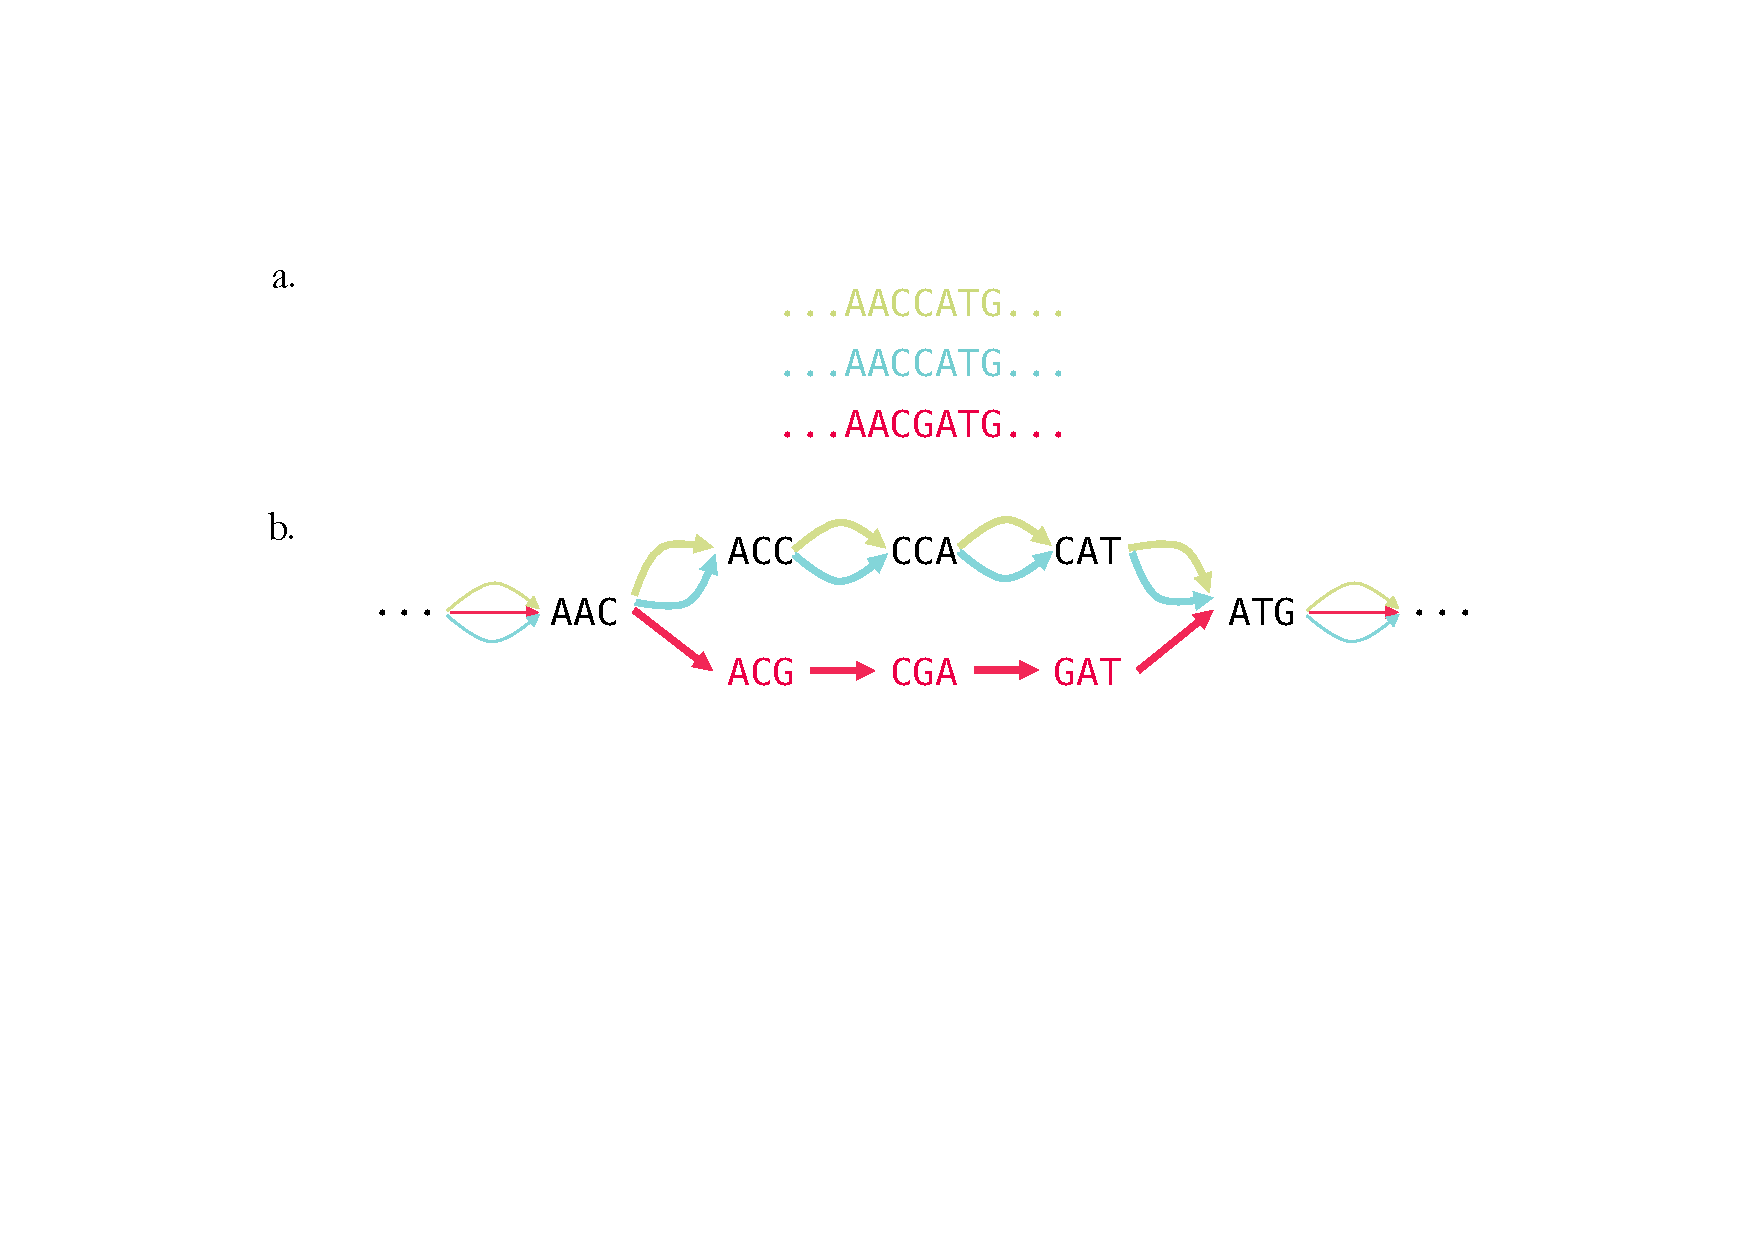
\includegraphics[width=\textwidth]{db_graph_cartoon}
  \caption{a. Haploid sequences from a mother (green), father (blue), and child (red), the last differing from the first two by a single SNP.  b. The resulting multi-color de Bruijn graph for $k=3$. Red vertices denote kmers that are deemed "novel", i.e. present in the child and absent in the parents. Edge colors reflect the samples in which the connected pairs of kmers are found. Edges that are part of the bubble (variant call) are displayed with thicker lines.}
  \label{fig:db_graph_cartoon}
\end{figure}

\begin{figure}[h!]
  \centering
    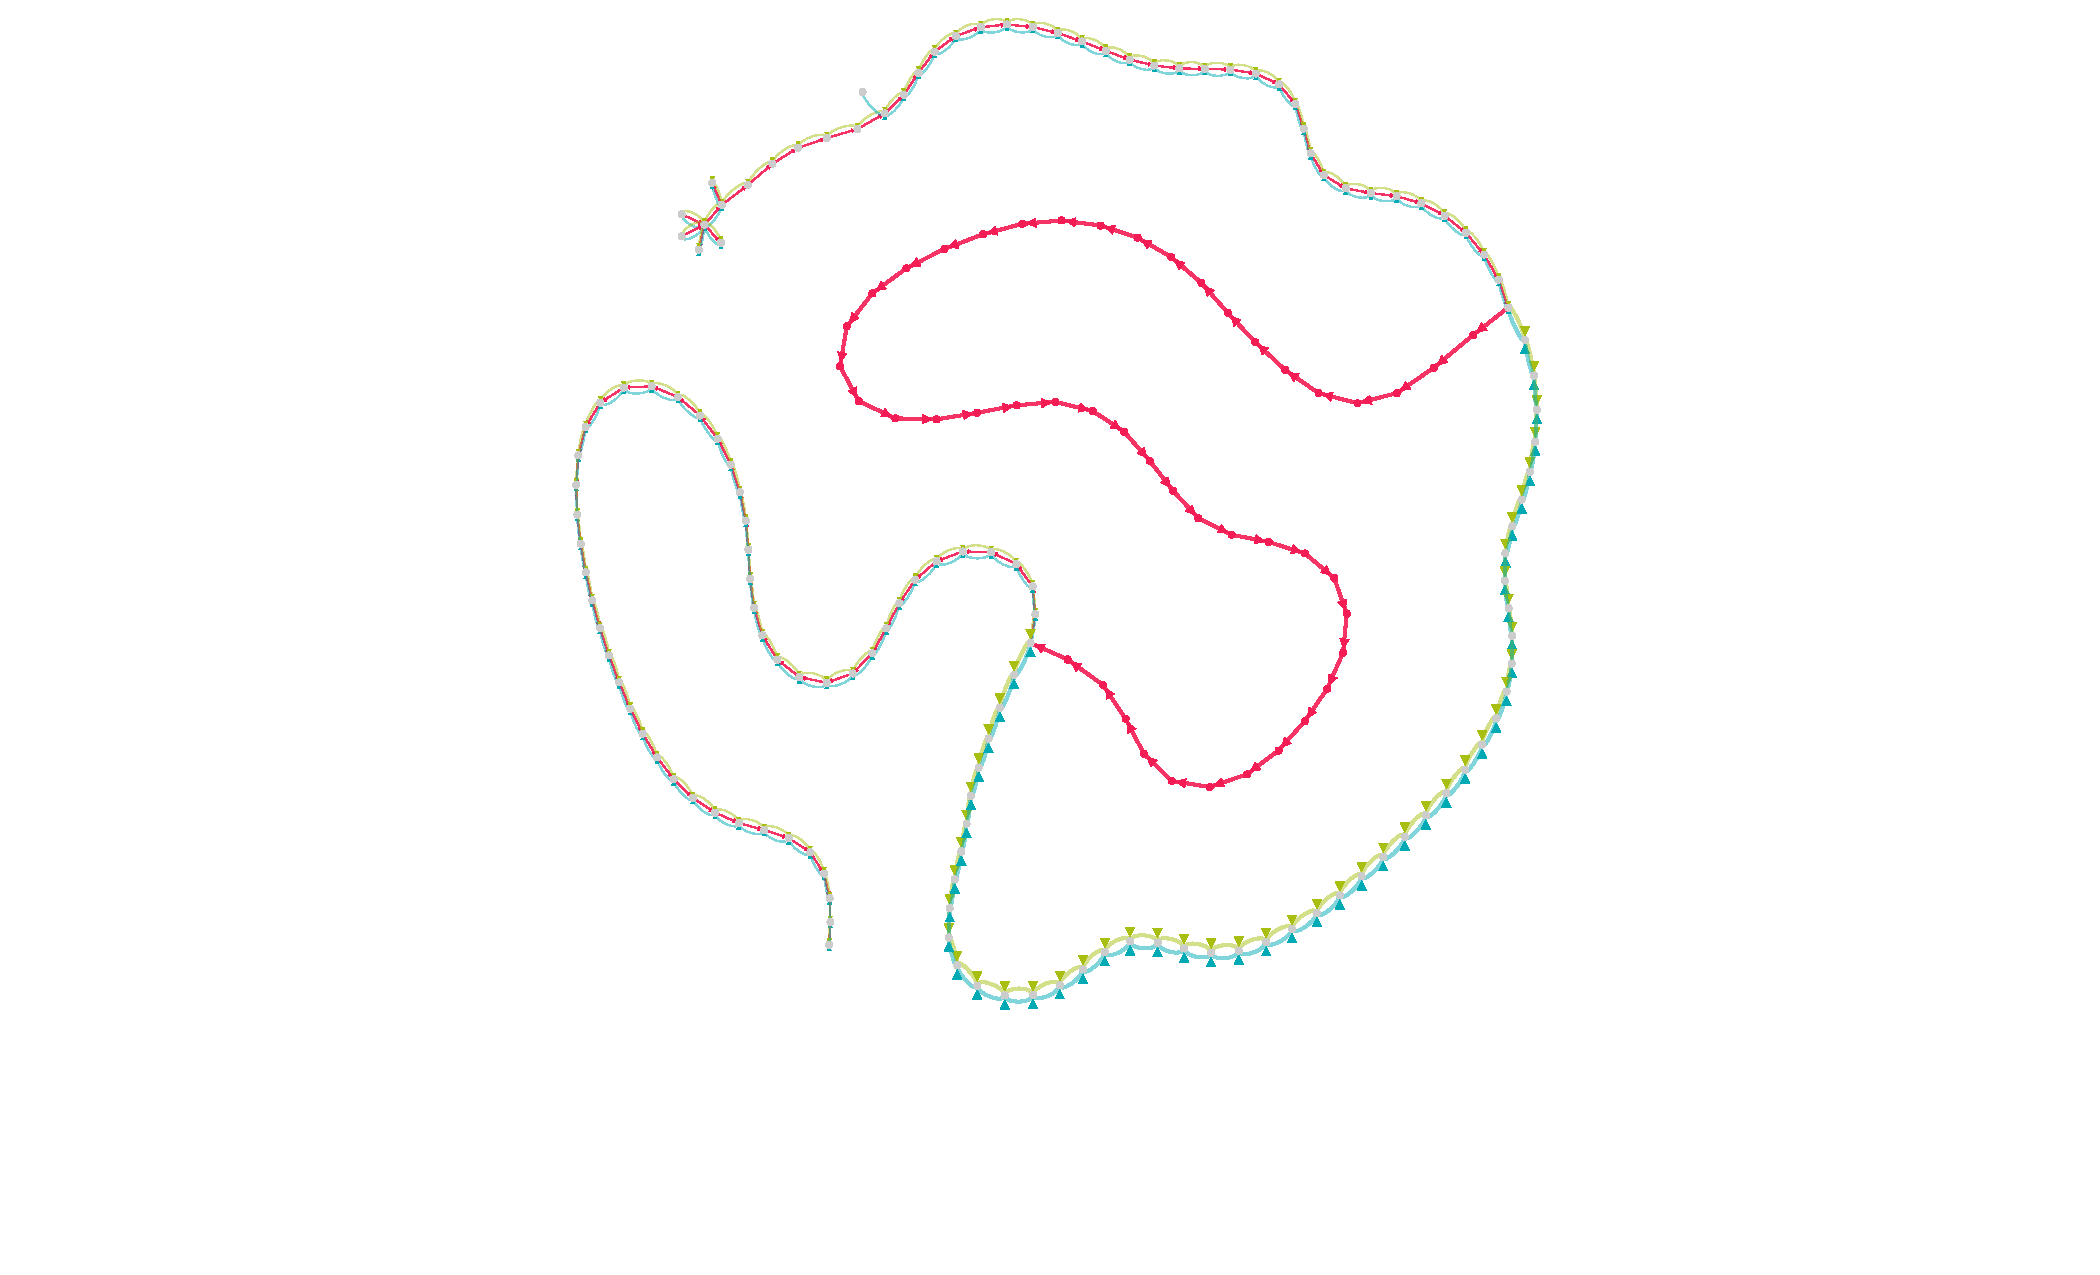
\includegraphics[width=0.5\textwidth]{snp_no_errors}
  \caption{A multi-color de Bruijn graph at $k=47$ for a haploid pedigree spanning a simulated \textit{de novo} SNP.  Vertex labels have been supressed for clarity.  Spatial layout is arbitrary and for display purposes only.}
  \label{fig:snp_no_errors}
\end{figure}

All simple variants will have this basic structure: a bubble in the graph that separates the variant samples from the non-variant samples.  The only major difference is the length of each branch: longer for an insertion in the child, shorter for a deletion (note that for short events, this is generally not apparent from the display, as evidenced by figures \ref{fig:ins_no_errors} and \ref{fig:del_no_errors}).

\begin{figure}[h!]
  \centering
    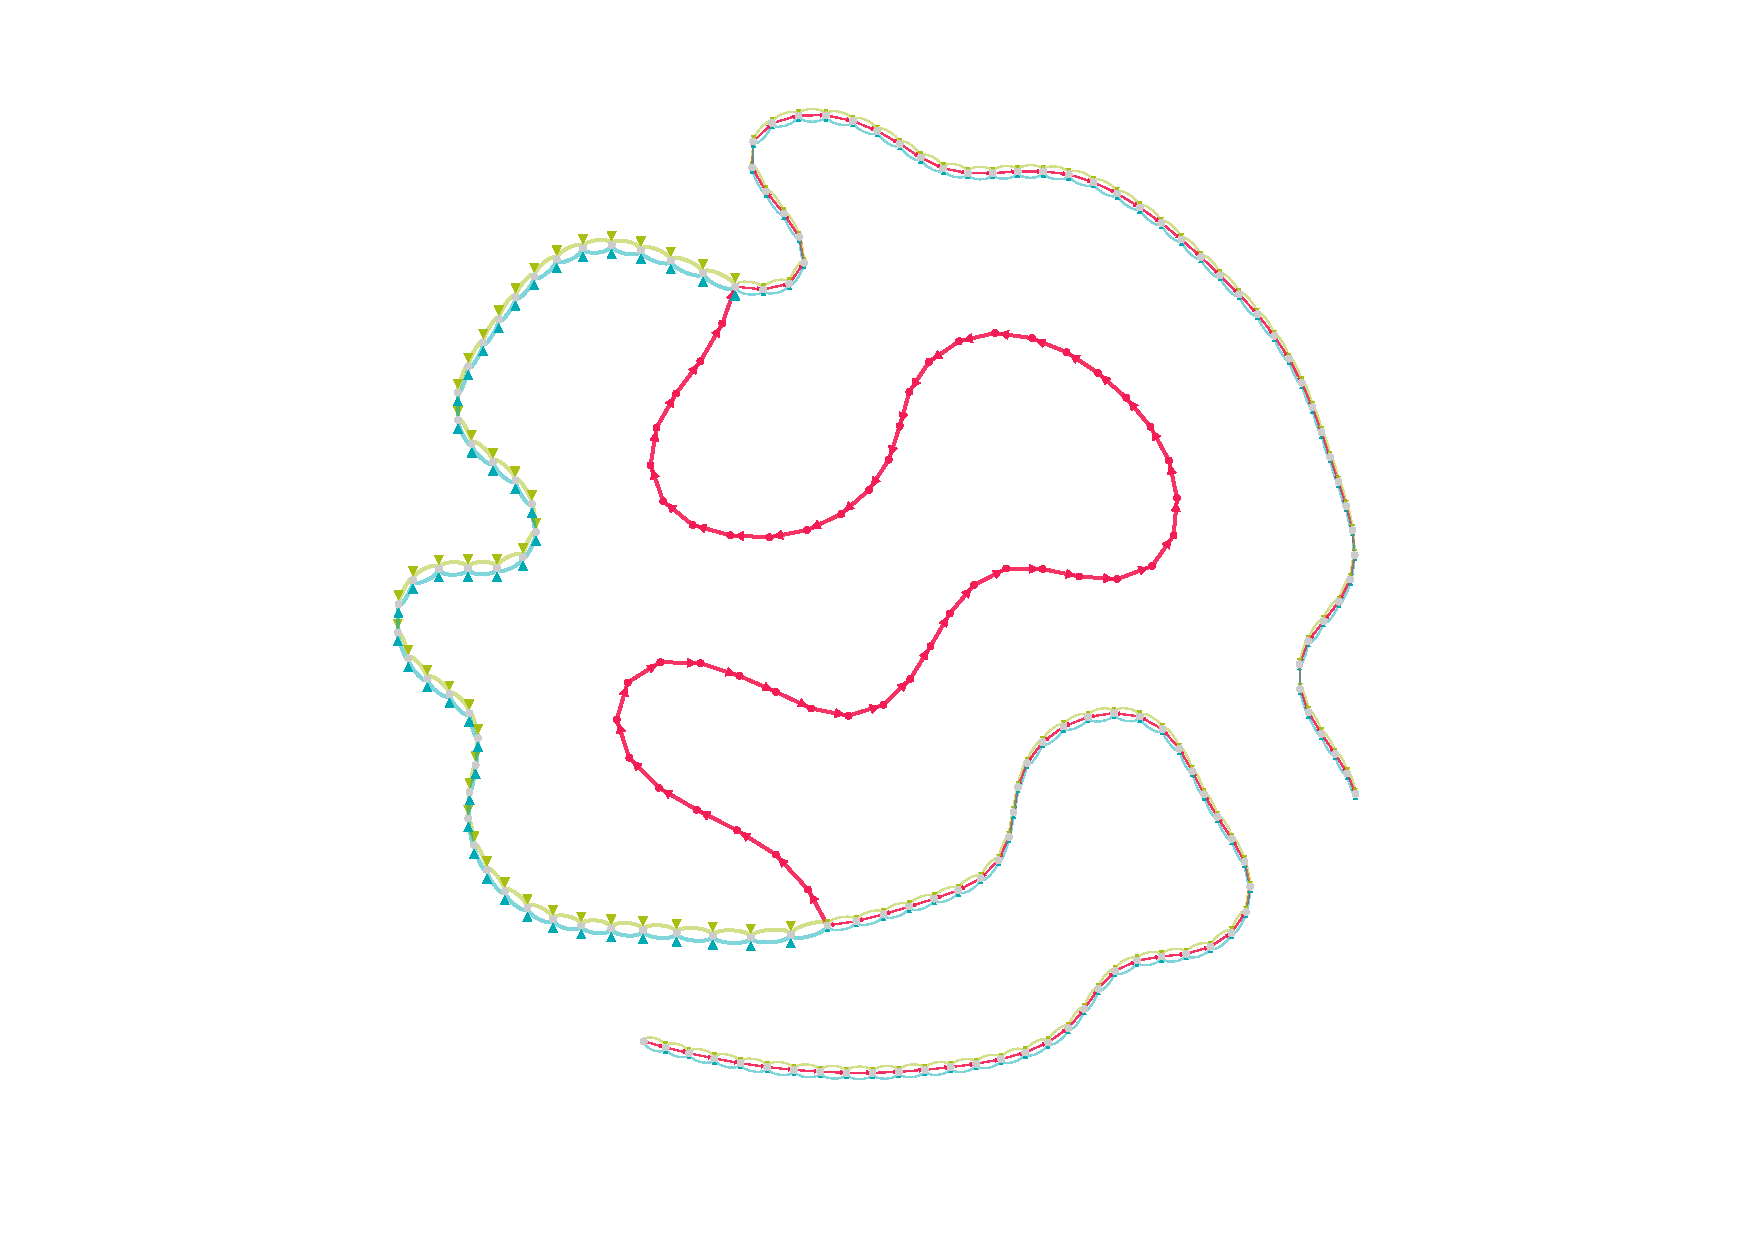
\includegraphics[width=0.5\textwidth]{ins_no_errors}
  \caption{A $5$ bp insertion in the child}
  \label{fig:ins_no_errors}
\end{figure}

\begin{figure}[h!]
  \centering
    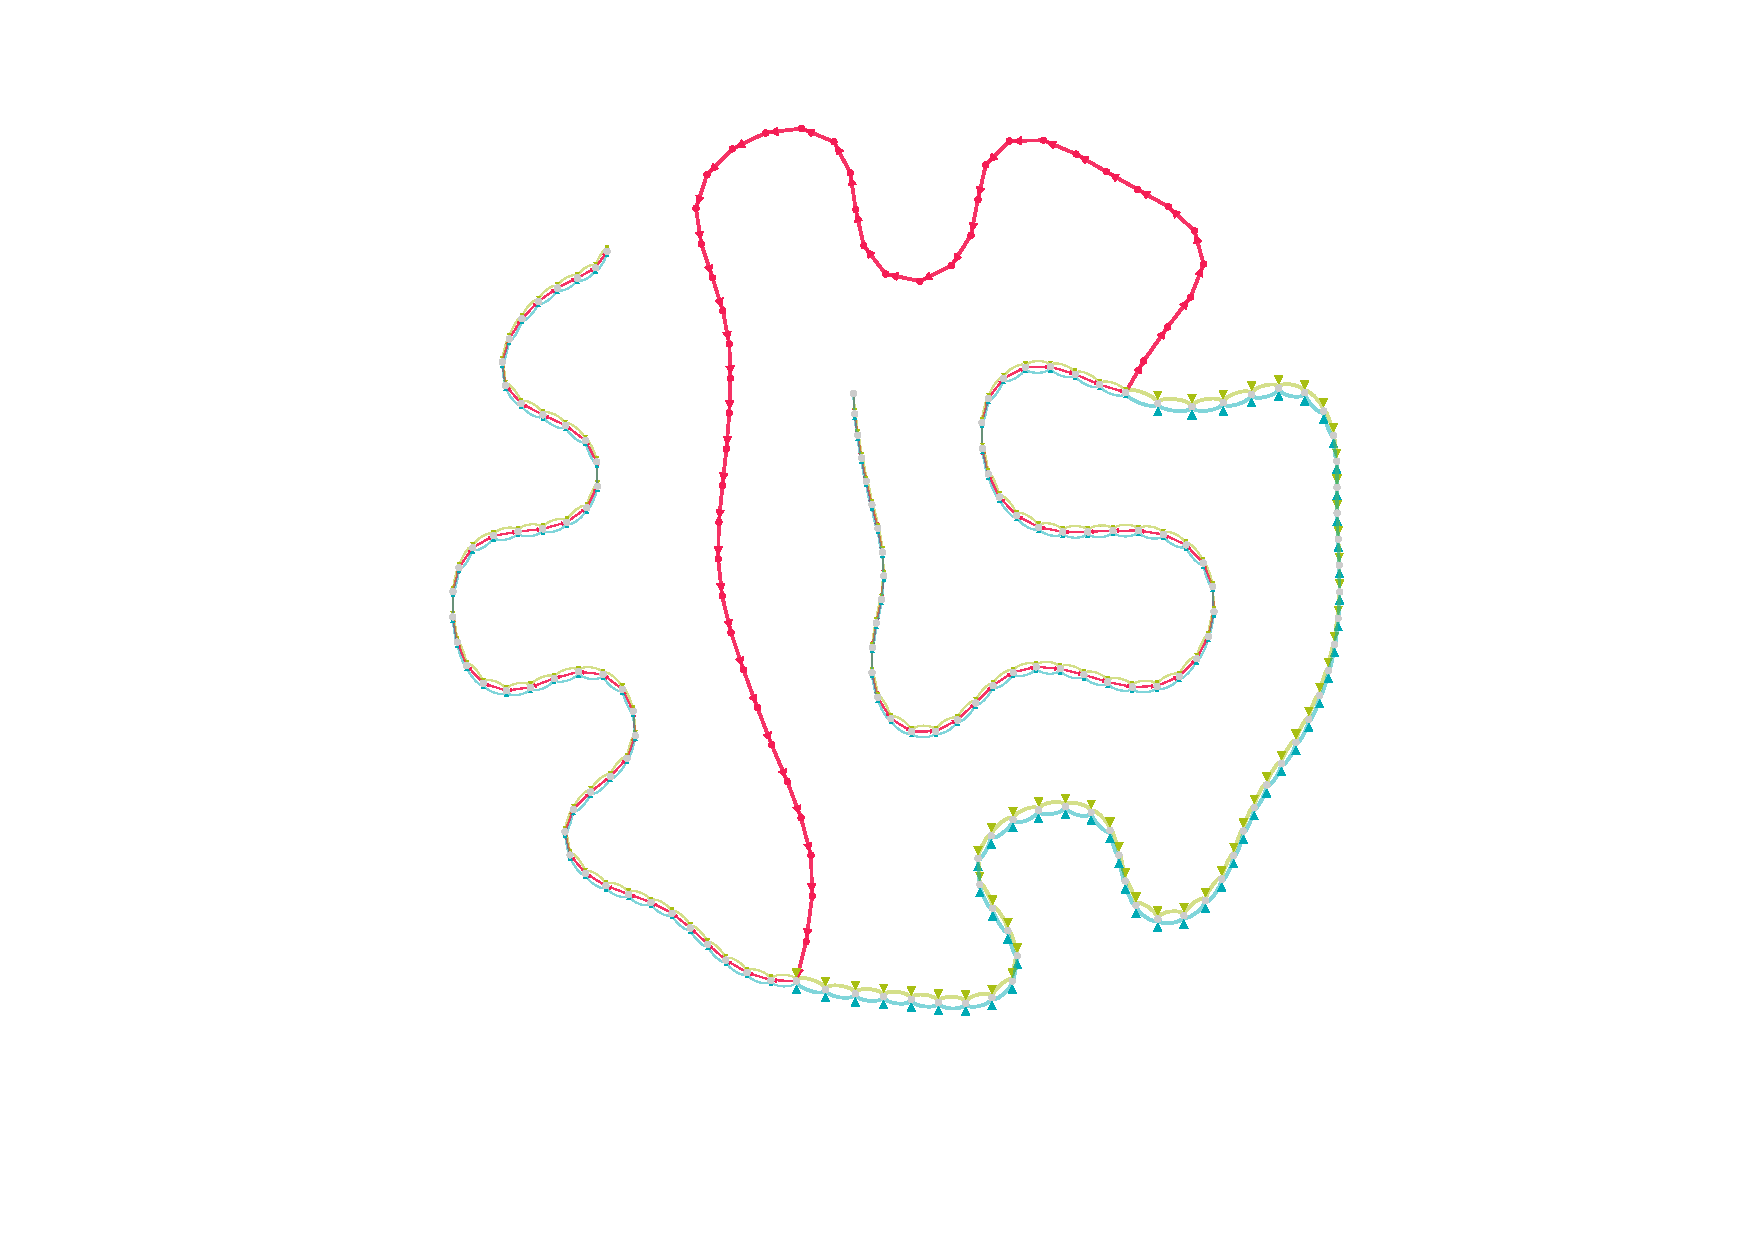
\includegraphics[width=0.5\textwidth]{del_no_errors}
  \caption{A $5$ bp deletion in the child}
  \label{fig:del_no_errors}
\end{figure}

The previous examples have all involved \textit{de novo} variants on perfectly homologous parental haplotypic backgrounds.  However, many variants may occur on the background of one parent or another.  Figure \ref{fig:td_haplotypic_background} depicts one such event.  A 41-bp tandem duplication has occurred on the background of the mother, as evidenced by the presence of green edges, but no blue edges.  In the flanking tails, edges shared between all three samples are present, until a blue edge separates from the graph and connects to different vertices.  While not shown, these branches continue along the genome of the father.

\begin{figure}[h!]
  \centering
    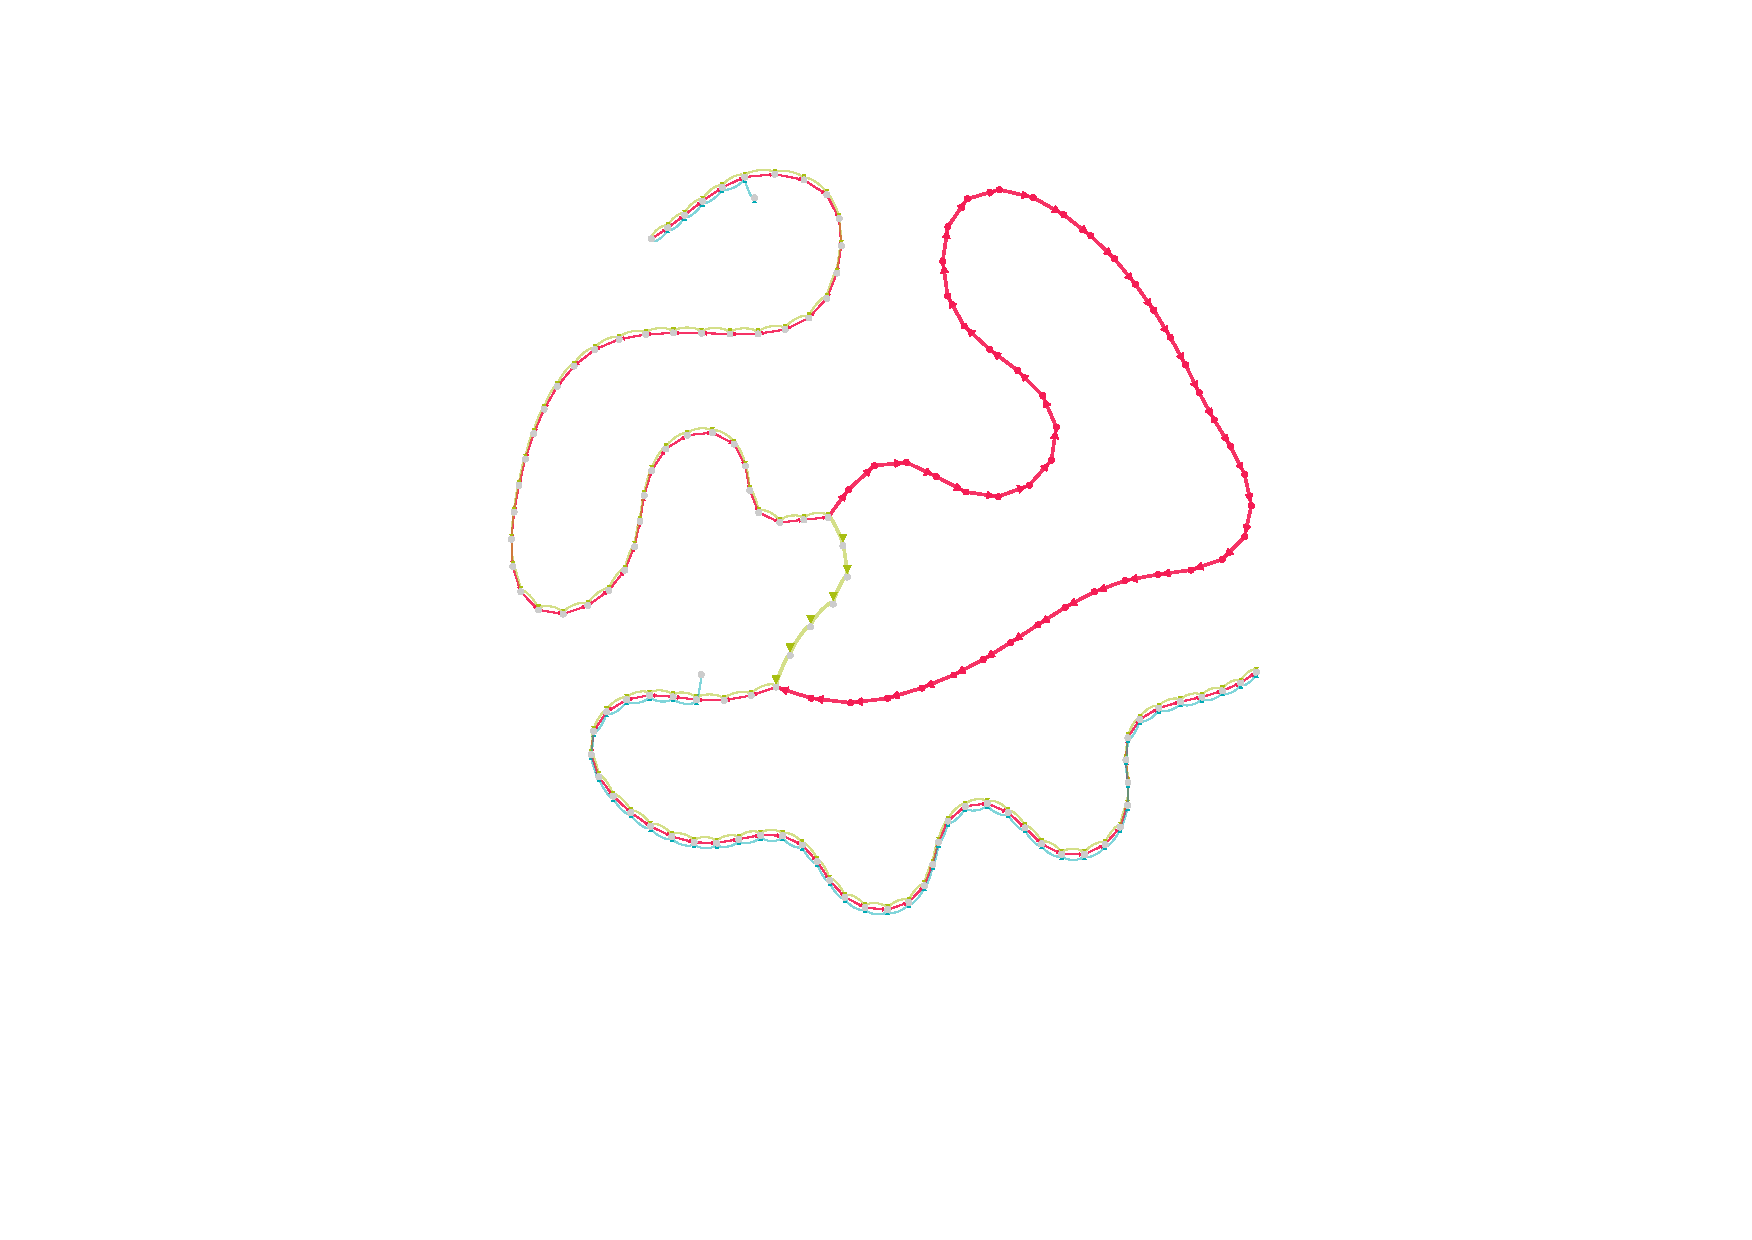
\includegraphics[width=0.5\textwidth]{td_haplotypic_background}
  \caption{A tandem duplication on the haplotypic background of the mother.}
  \label{fig:td_haplotypic_background}
\end{figure}

Finally, it is possible to encounter variants where the path through the graph taken by the child can appear to follow both the variant and non-variant paths, as demonstrated by figure \ref{fig:inv_child_follows_parents}.  Such a scenario may arise by a mutation on a sequence with copy number greater than $1$: both the unaltered and altered sequences would then exist simultaneously in the child's genome.

\begin{figure}[h!]
  \centering
    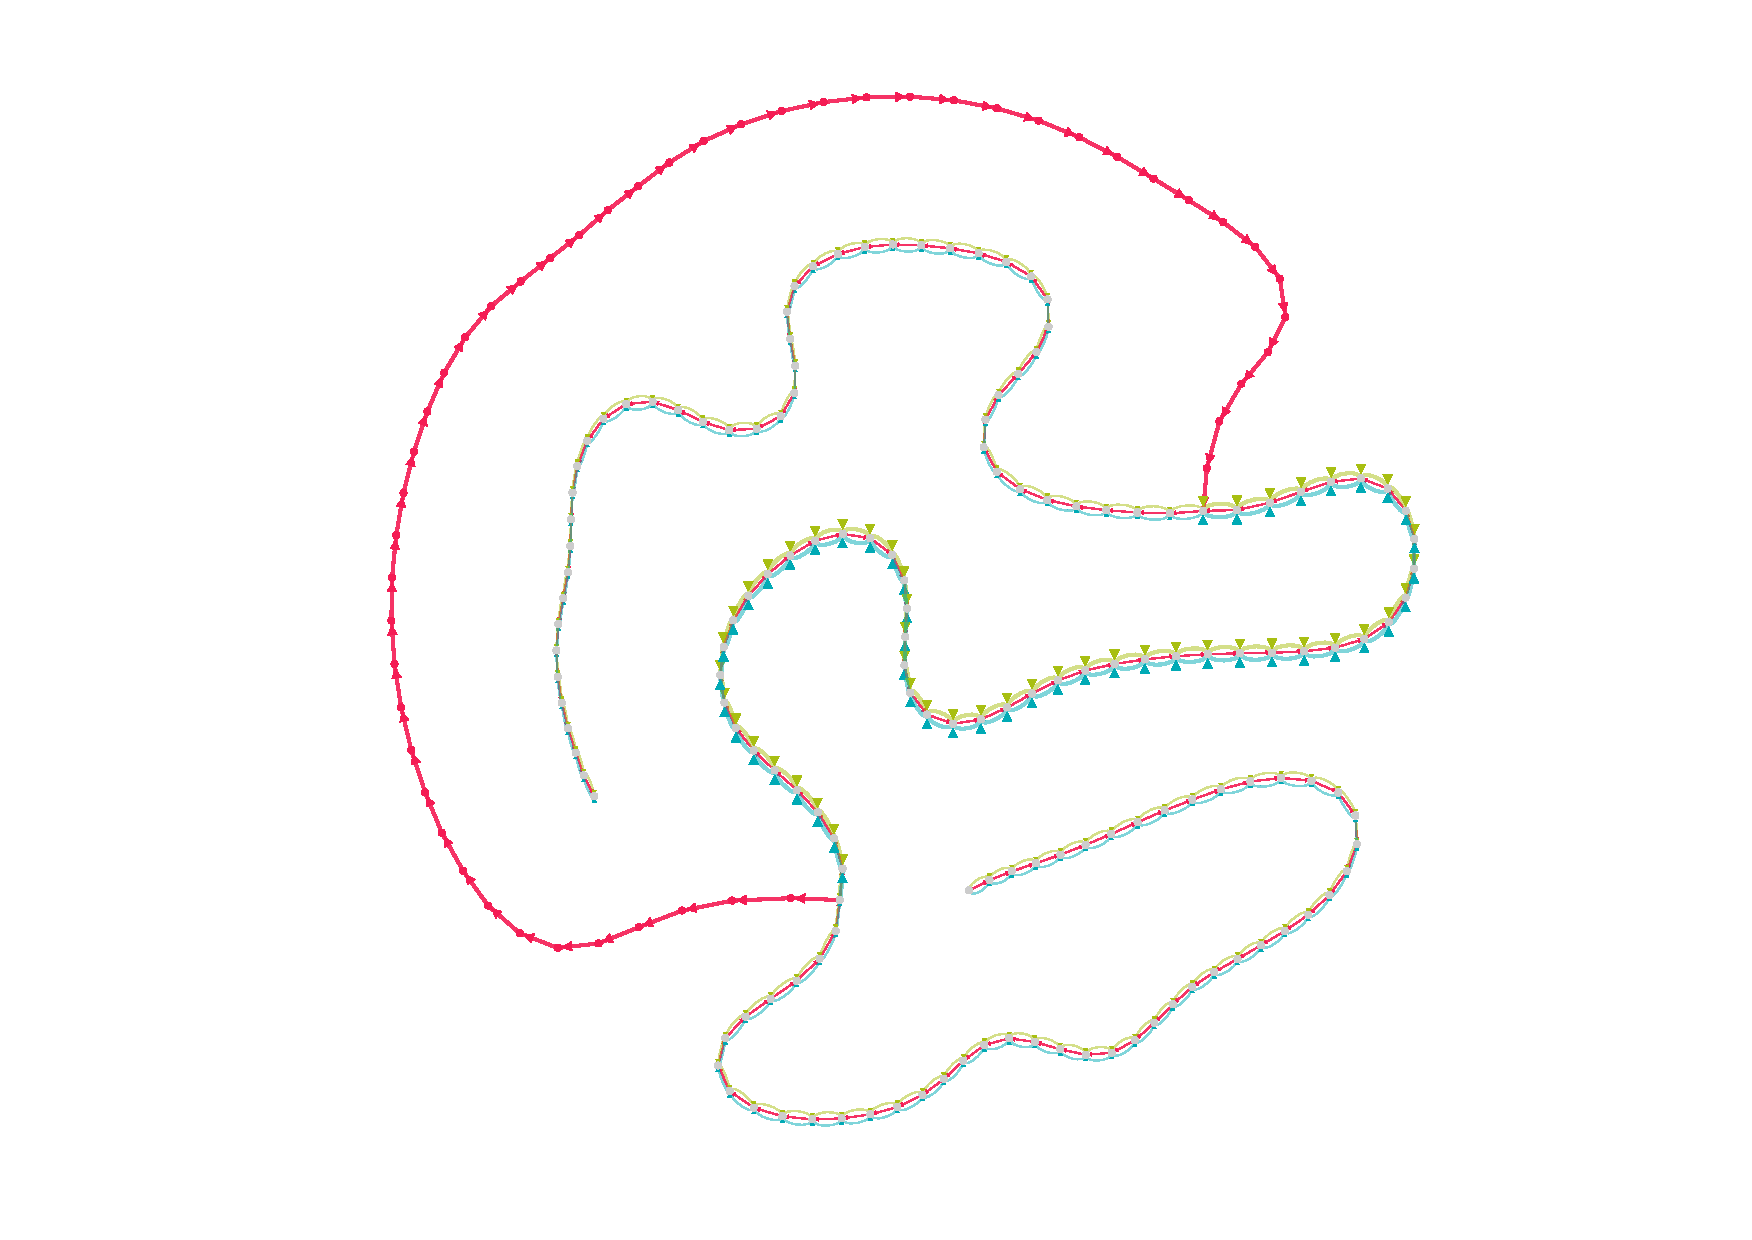
\includegraphics[width=0.5\textwidth]{inv_child_follows_parents}
  \caption{A variant wherein the child's path does not simply diverge from that of the parents, but rather navigates both.}
  \label{fig:inv_child_follows_parents}
\end{figure}

\subsection{Complex variant motifs}
